\documentclass[12pt]{exam}

% essential packages
\usepackage{fullpage} % margin formatting
\usepackage{enumitem} % configure enumerate and itemize
\usepackage{amsmath, amsfonts, amssymb, mathtools} % math symbols
\usepackage{xcolor, colortbl} % colors, including in tables
\usepackage{makecell} % thicker \Xhline in table
\usepackage{graphicx} % images, resizing

% sometimes needed packages
\usepackage{hyperref} % hyperlinks
\usepackage{tikz} % drawing graphs
\usetikzlibrary{positioning}

% paragraph formatting
\setlength{\parskip}{6pt}
\setlength{\parindent}{0cm}

% newline after Solution:
\renewcommand{\solutiontitle}{\noindent\textbf{Solution:}\par\noindent}

% less space before itemize/enumerate
\setlist{topsep=0pt}

% creates \filcl to grey out cells for groupwork grading
\newcommand{\filcl}{\cellcolor{gray!25}}

% creates \probnum to get the problem number
\newcounter{probnumcount}
\setcounter{probnumcount}{1}
\newcommand{\probnum}{\arabic{probnumcount}. \addtocounter{probnumcount}{1}}

% use roman numerals by default
\setlist[enumerate]{label={(\roman*)}}

% creates custom list environments for grading guidelines, question parts
\newlist{guidelines}{itemize}{1}
\setlist[guidelines]{label={}, left=0pt .. \parindent, nosep}
\newlist{gwguidelines}{enumerate}{1}
\setlist[gwguidelines]{label={(\roman*)}, nosep}
\newlist{qparts}{enumerate}{2}
\setlist[qparts]{label={(\alph*)}}
\newlist{qsubparts}{enumerate}{2}
\setlist[qsubparts]{label={(\roman*)}}
\newlist{stmts}{enumerate}{1}
\setlist[stmts]{label={(\roman*)}, nosep}
\newlist{pflist}{itemize}{4}
\setlist[pflist]{label={$\bullet$}, nosep}
\newlist{enumpflist}{enumerate}{4}
\setlist[enumpflist]{label={(\arabic*)}, nosep}

\printanswers

\newcommand{\prevhwnum}{7}
\newcommand{\hwnum}{8}

\begin{document}
%%%%%%%%%%%%%%% TITLE PAGE %%%%%%%%%%%%%%%
\title{EECS 203: Discrete Mathematics\\
	Winter 2024\\
	Homework \hwnum{}}
\date{}
\author{}
\maketitle
\vspace{-50pt}
\begin{center}
	\huge Due \textbf{Thursday, April 4}, 10:00 pm\\
	\Large No late homework accepted past midnight.\\
	\vspace{10pt}
	\large Number of Problems: $8+2$
	\hspace{3cm}
	Total Points: $100+30$
\end{center}
\vspace{25pt}
\begin{itemize}
	\item \textbf{Match your pages!} Your submission time is when you upload the file, so the time you take to match pages doesn't count against you.
	\item Submit this assignment (and any regrade requests later) on Gradescope.
	\item Justify your answers and show your work (unless a question says otherwise).
	\item By submitting this homework, you agree that you are in compliance with the Engineering Honor Code and the Course Policies for 203, and that you are submitting your own work.
	\item Check the syllabus for full details.
\end{itemize}
\newpage
%%%%%%%%%%%%%%% TITLE PAGE %%%%%%%%%%%%%%% 

\section*{Individual Portion}

\subsection*{\probnum Easy Peasy Degree-sy Squeezy [8 points]}
Let $G$ be a graph with $v$ vertices and $e$ edges. Let $M$ be the maximum degree of the vertices of $G$, and let $m$ be the minimum degree of the vertices of $G$. Show that
\begin{qparts}
	\item $\dfrac{2e}{v} \geq m$
	\item $\dfrac{2e}{v} \leq M$
\end{qparts}


% the formula is 2e=\sum_{v \in V} \text{deg}(v)
% since we set the exact degree of a vertex to d, substitute d for \text{deg}(v)
% so the formula becomes 2e=\sum_{v \in V} d
\begin{solution}

	a) By the Handshaking Theorem, we know that the sum of the degrees of all the vertices in a graph is equal to twice the number of edges in the graph. That is, $\sum_{v \in V} \text{deg}(v) = 2|E|$. We can use this fact to prove the two inequalities.
	Since $m$ is the minimum degree of the vertices of $G$, we know that $m \leq \text{deg}(v) \leq M$ for all $v \in V$. Then, we have the following:
	\begin{align*}
		2|E|              & \geq \sum_{v \in V} m \\
		2|E|              & \geq m|V|             \\
		2|E|              & \geq m|V|             \\
		\dfrac{2|E|}{|V|} & \geq m
	\end{align*}
	\\b)
	\begin{align*}
		2|E|              & \leq \sum_{v \in V} M \\
		2|E|              & \leq M|V|             \\
		2|E|              & \leq M|V|             \\
		\dfrac{2|E|}{|V|} & \leq M
	\end{align*}
	This proves the second inequality. Thus, we have shown that $\dfrac{2e}{v} \geq m$ and $\dfrac{2e}{v} \leq M$.
	Therefore, $\dfrac{2e}{v} \geq m$ and $\dfrac{2e}{v} \leq M$.
\end{solution}

\subsection*{\probnum The Forest Beyond the Trees [15 points]}
Determine which of the following graphs is/are a tree. Additionally, determine which of the following graphs is/are bipartite. Please explain your reasoning for why each one is or is not a tree, and why each one is or is not bipartite.
\begin{qparts}
	\item $C_4,$ a cycle of length 4
	\item ~\\
	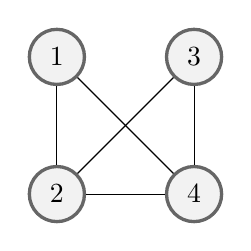
\begin{tikzpicture}[
			roundnode/.style={circle, draw=black!60, fill=gray!10, very thick, minimum size=7mm},
		]
		%Nodes
		\node[roundnode] (1) {1};
		\node[roundnode] (2) [below=of 1] {2};
		\node[roundnode] (3) [right=of 1] {3};
		\node[roundnode] (4) [below=of 3] {4};

		\draw[-] (3)--(4);
		\draw[-] (2)--(3);
		\draw[-] (4)--(2);
		\draw[-] (2)--(1);
		\draw[-] (1)--(4);
	\end{tikzpicture}

	\item $K_6$
	\newpage
	\item ~\\\includegraphics[scale = 0.4]{Homework/Images/treebipartitesecond.png}
	\item ~\\\includegraphics[scale = 0.4]{Homework/Images/treebipartite.png}
\end{qparts}

% for this, write out tree, and bipartite definitions respectively
\begin{solution}
	a) A tree is a connected graph with no cycles. Since $C_4$ is a cycle of length 4, it is not a tree.\\
	It is bipartite because the graph can be divided into two disjoint sets such that no two vertices within the same set are adjacent.\\
	b) It is not a tree because $(1,4,2,1)$ is a simple circuit.\\
	It is not bipartite because 1 is adjacent to both 2 and 4, it is impossible to color those with two colors such that the graph is bipartite.\\
	c) It is not a tree nor bipartite.\\
	This is because $K_6$ has multiple cycles, and it is not possible to divide the vertices into two disjoint sets such that no two vertices within the same set are adjacent.\\
	d) A tree is a connected graph with no cycles. Since the graph is connected and has no cycles, it is a tree.\\
	A bipartite graph is a graph whose vertices can be divided into two disjoint sets such that no two vertices within the same set are adjacent. Since the graph can be divided into two disjoint sets such that no two vertices within the same set are adjacent, it is bipartite.\\
	e) It is not a tree because$c$ is not connected with the rest of the graph.\\
	It is bipartite because the graph can be divided into two disjoint sets such that no two vertices within the same set are adjacent.\\
	i.e. $(a,c,e,g,i)$ and $(b,d,f,h)$ can be the two disjoint sets.

\end{solution}

\newpage
\subsection*{\probnum Road Rage [12 points]}
The graphs below shows some major roads in New Jersey. The graph on the left shows distances between cities on these roads, and the graph on the right shows the toll costs on each road.

\resizebox{\textwidth}{!}{
	\includegraphics[]{Homework/Images/njroads.png} \includegraphics[]{Homework/Images/njtolls.png}
}

For each pair of cities below, (i) find the shortest path in distance, and (ii) find the least expensive route (shortest path in terms of cost). Be sure to list the total distance and total cost for each respective part.

\begin{qparts}
	\item Newark to Camden
	\item Trenton to Atlantic City
\end{qparts}

\begin{solution}
	a) i) Newark to Camden\\
	The shortest path in distance from Newark to Camden is Newark $\rightarrow$ Woodbridge $\rightarrow$ Camden. The total distance is 80 miles.\\
	ii)
	The least expensive route from Newark to Camden is Newark $\rightarrow$ Woodbridge $\rightarrow$ Camden. The total cost is $0.60+0=0.60$ dollars.\\
	\\b) i) Trenton to Atlantic City\\
	The shortest path in distance from Trenton to Atlantic City is Trenton $\rightarrow$ Camden $\rightarrow$ Atlantic City. The total distance is 86 miles.\\
	ii) The least expensive route from Trenton to Atlantic City is Trenton $\rightarrow$ Asbury Park $\rightarrow$ Atlantic City. The total cost is $0+1.25=1.25$ dollars.
\end{solution}

\newpage
\subsection*{\probnum Isomorphish? [12 points]}
Determine whether or not each of the following pairs of graphs are isomorphic. If yes, provide an isomorphism. If not, explain why and propose a change to one of the graphs that would make them isomorphic; you do not need to provide an isomorphism in this case.
\begin{qparts}
	\item ~\\\includegraphics[]{Homework/Images/isomorphisim_graph_1.png} \includegraphics[]{Homework/Images/isomorphisim_graph_2.png}
	\item ~\\\includegraphics[scale=.85]{Homework/Images/isomorphisim_graph_4.png} \includegraphics[scale=.85]{Homework/Images/isomorphisim_graph_3.png}
\end{qparts}

\begin{solution}
	a) The two graphs are isomorphic. The isomorphism is as follows:
	Let $f$ be\\
	$f(a) = 1$\\
	$f(b) = 4$\\
	$f(c) = 0$\\
	$f(d) = 3$\\
	$f(e) = 2$\\
	b) The two graphs are not isomorphic. \\
	The first graph has 1 vertex of degree 5, 2 vertices of degree 4, 1 vertex of degree 3, and 3 vertices of degree 2.\\
	The second graph has 2 vertices of degree 5, 2 vertices of degree 4, and 3 vertices of degree 2.\\
	To make them isomorphic, we can remove an edge between $a$ and $c$ in the second graph. This will make the second graph have 1 vertex of degree 5, 2 vertices of degree 4, 1 vertex of degree 3, and 3 vertices of degree 2.\\


\end{solution}

\newpage

\subsection*{\probnum Any tours available? [12 points]}
State whether each of the following contains, or is guaranteed to contain a Hamiltonian Cycle. Justify your response for each part.
\begin{qparts}
	\item ~\\\includegraphics[width=3cm]{Homework/Images/hamcycle_a.png}
	\item ~\\\includegraphics[width=7.5cm]{Homework/Images/hamcycle_b.png}
	\item A simple, bipartite graph with 4 vertices that contains one cycle
	\item A 4-vertex graph where each vertex has even degree
\end{qparts}

\begin{solution}
	a) The graph contains a Hamiltonian Cycle. The Hamiltonian Cycle is as follows: $a \rightarrow b \rightarrow c \rightarrow d \rightarrow e \rightarrow a$.\\
	It is not guaranteed to contain a Hamiltonian Cycle because to get from $a$ to $e$, we can go $a\rightarrow e$.
	\\b) The graph does not contain a Hamiltonian Cycle because there is only one way to go from $a,b$ side to $c,d$ side and back.\\
	c) It is guaranteed to contain a Hamiltonian Cycle. Since it is a simple graph with 4 vertices that contains one cycle, the Hamiltonian Cycle is as follows: $a \rightarrow b \rightarrow c \rightarrow d \rightarrow a$.\\
	d) It is not guaranteed to contain a Hamiltonian Cycle. The graph is a 4-vertex graph where each vertex has even degree, including $0$. However, the graph is not guaranteed to be connected, so it does not contain a Hamiltonian Cycle.
\end{solution}

\newpage
\subsection*{\probnum Euler Visits the U.S. [12 points]}
Let $G=(V,E)$ be a graph of the continental U.S. where $V$ is the set of the first 48 states (excluding Alaska and Hawaii) and $E$ contains all pairs that share a border.  (Arizona and Colorado do not share a border, nor do Utah and New Mexico). A reference for the U.S. map has been provided below.

\begin{center}
	~\\\includegraphics[width=15cm]
	{Homework/Images/USMap1.png}
\end{center}

\begin{qparts}
	\item Does $G$ have an Euler path?  Prove or disprove.

	\item Is $G$ 3-colorable?  In other words, is there a function $f\colon V\rightarrow\{\text{red,blue,green}\}$ such that if $\{u,v\}\in E$ then $f(u)\neq f(v)$?

	\textbf{Hint:} Consider odd wheels $W_{2k + 1}$
\end{qparts}

\begin{solution}
	a) Disproof:\\
	The Euler Theorem states that a connected graph has an Euler path if and only if it has exactly 0 or 2 vertices of odd degree. Since the graph of the continental U.S. has 48 vertices, and each state shares a border with at least one other state, each state has an even degree. However, there are at least $3$ states that have an odd degree, which are Nevada, Louisiana. and Kentucky. Therefore, the graph does not have an Euler path.\\
	b) $G$ is not 3-colorable.\\
	Consider the odd wheel $W_3$. The odd wheel $W_3$ is a graph with 3 vertices, where each vertex is connected to the other two vertices. The odd wheel $W_3$ is not 3-colorable because each vertex is connected to the other two vertices, so each vertex must have a different color from the other two vertices. This is the same case for the graph of the continental U.S. because in a) we found that there are at least 3 states that have an odd degree. Therefore, the graph is not 3-colorable.\\
	We can also use the Pigeonhole Principle. Let the Pigeons be any state with more than 2 neighbors, and the holes be the 3 colors. Since each state has at most 3 neighbors, we can color each state with 3 colors. However, since there are at least 3 states with more than 2 neighbors, we cannot color the graph with 3 colors. Therefore, the graph is not 3-colorable.

\end{solution}

\newpage
\subsection*{\probnum Ham and Cheese [15 points]}
A Hamiltonian cycle is a cycle that traverses through every vertex in a graph exactly once (starting and ending at the same vertex). How many Hamiltonian cycles are there in the complete graph $K_n$? Justify your answer.

\textbf{Note:} Two cycles are the same as long as the have the same vertices, and each vertex has the same left and right neighbors in the cycle. For instance the cycles $(a,b,c,a),$ $(b,c,a,b),$ and $(a,c,b,a)$ are all equivalent.

\begin{solution}
	For a complete graph $K_n$, there are $\frac{n!}{2n}=\frac{(n-1)!}{2}$ Hamiltonian cycles.\\
	We start with $n$ vertices, and we can choose any of the $n$ vertices to start with.\\
	Then, we have $n-1$ choices for the next vertex, $n-2$ choices for the next vertex, and so on.\\
	However, we have to divide by $n$ because the cycle can start at any of the $n$ vertices with the same left and right neighbors, and we have to divide by $2$ because the cycle can be traversed in either direction (backward or forward).\\
	Therefore, there are $\frac{n!}{2n}=\frac{(n-1)!}{2}$ Hamiltonian cycles in the complete graph $K_n$.

\end{solution}

\subsection*{\probnum Captivating Counts [14 points]}
How many positive integers between $1000$ and $9999$ inclusive
\begin{qparts}
	\item have distinct digits?
	\item are divisible by 5 or 7?
	\item are divisible by 5 but not by 7?
\end{qparts}
Justify \textbf{and simplify} your answers. You may use a calculator to simplify.

\begin{solution}
	Let the universe be $U = \{1000,1001,...,9999\}$.\\
	Define $S_k = \{x \in U : k | x\}$ to be the multiples of $k$ in $U$.\\
	Let $n$ be the last number in the set, we break down the set into groups of $k$ since from $1$ to $n$, there are $\left\lfloor \dfrac{n}{k} \right\rfloor$ multiples of $k$.\\
	\begin{align}
		|S_5|          & = \left\lfloor \dfrac{9999}{5} \right\rfloor - \left\lfloor \dfrac{1000}{5} \right\rfloor = 1999 - 200 + 1= 1800 \\
		|S_7|          & = \left\lfloor \dfrac{9999}{7} \right\rfloor - \left\lfloor \dfrac{1000}{7} \right\rfloor = 1428 - 142 = 1286    \\
		|S_5 \cap S_7| & = \left\lfloor \dfrac{9999}{35} \right\rfloor - \left\lfloor \dfrac{1000}{35} \right\rfloor = 285 - 28 = 257     \\
	\end{align}

	a) $9\cdot 9\cdot 8\cdot 7 = 4536$\\
	There are 4 digits in the number, and the first digit cannot be 0.\\
	There are $9$ choices for the first digit, $9$ choices for the second digit, $8$ choices for the third digit, and $7$ choices for the fourth digit.\\
	b) The question is asking for $|S_5 \cup S_7|$.\\
	\begin{align}
		|S_5 \cup S_7| = |S_5| + |S_7| - |S_5 \cap S_7| = 1800 + 1286 - 257 = 2829 \\
	\end{align}
	c) The question is asking for $|S_5 - S_7|$.
	\begin{align}
		|S_5 - S_7| & = |S_5| - |S_5 \cap S_7| = 1800 - 257 = 1543 \\
	\end{align}
\end{solution}
\end{document}
